\documentclass[man]{apa6}
%%%Packages 
\usepackage{apacite}  % apacite
\usepackage{amssymb, amsmath, amsthm} % symbols and math
\usepackage{graphicx, latexsym}
\usepackage{bibentry} % om referentie in text te kunnen gebruiken
\usepackage{cancel} % for cancel function

\usepackage{apacite}
%\usepackage{natbib}

\usepackage{tcolorbox} 
\captionsetup[figure]{belowskip=0pt,aboveskip=12pt,labelfont=it,textfont={normal},labelsep=period,singlelinecheck=off,justification=raggedright}
\captionsetup[table]{belowskip=12pt,aboveskip=12pt,labelfont=normal,textfont={it},labelsep=newline,singlelinecheck=off,justification=centering}

\title{Staying in the loop. Prior odds, Bayes factor, Posterior Odds}
\shorttitle{Staying in the loop}
%%%% paper title
\author{Fayette Klaassen}
\affiliation{Department of Methodology and Statistics, Utrecht University, The Netherlands}
\authornote{Correspondence should be addressed to Fayette Klaassen, Department of Methodology and Statistics, Utrecht University, P.O. Box 80140, 3508 TC Utrecht, The Netherlands. E-mail: \textsf{f.klaassen@uu.nl}. This research was supported by a grant from The Netherlands Organisation for Scientific Research (NWO): NWO 406-12-001.}
\date{\today}
\abstract{
Bayesian hypothesis testing makes use of the Bayes factor, a quantification of the relative evidence for two hypotheses.
Following Bayes' theorem, a Bayes factor can be used to update prior odds (relative prior probabilities) of hypotheses into posterior odds.
Updating allows us to move from statements about the probability of \textit{data} given hypotheses, to statements about the probabilities of \textit{hypotheses} given the data.
Literature on how to specify prior probabilities is sparse and a practical definition of what a prior probability is lacks.
As a result, often no or equal prior probabilities are considered.
Alternatively, the Bayes factors is reported as the increase in prior odds and the reader is invited to update their own prior probabilities.
Existing literature on prior probabilities encompasses different (combinations of) these concepts and often lacks a practical approach.
This paper develops a definition of prior probabilities using three concepts: possibility, plausibility and value of a hypothesis.
Additionally, an elicitation procedure developed based on these concepts is introduced.
The results of the elicitation among ten behavioural researchers are discussed to illustrate two conclusions.
First, the procedure can be used to elicit different responses related to the possibility, plausibility and value of hypotheses, validating the definition.
Second, researchers are able to define prior probabilities following the procedure, validating it as a tool.
}
\keywords{Bayes factor; Posterior Odds; Prior odds; Replication; Updating}

\begin{document}
	
\maketitle
\section{Introduction}
%% updating in science
Updating knowledge is a key part of scientific research.
One of the first concepts discussed in any introductory methodology and statistics course is the scientific cycle \cite<e.g.>[p.14-18]{neuman11}, that discusses the updating of theories.
Theory and observations form the basis for new research questions and hypotheses.
By collecting and analyzing data, researchers try to answer these questions.
From this new state of knowledge theories can be further verified, fine-tuned or used to inform policy.
Continuously going through this cycle ensures that you are `staying in the loop'.
Updating is at the foundation of Bayesian statistics, visible in Bayes' theorem:
\begin{align}
\label{eq:BayesTheorem}
& P(A|D) = \dfrac{P(A) \times P(D|A)}{P(D)} \propto P(A) \times P(D|A)
\end{align}
that demonstrates how we can update our prior knowledge $P(A)$ about property $A$ with data $D$ into posterior knowledge $P(A|D)$ about $A$, conditional on $D$.
Equation~\ref{eq:BayesTheorem} is used to updated knowledge about parameters or hypotheses (substitute $\theta$ or $H$ for $A$, respectively).
Figure~\ref{fig:loops} illustrates updating at the level of theories, hypothesis probabilities and parameter distributions.
\begin{figure}
	\centering
	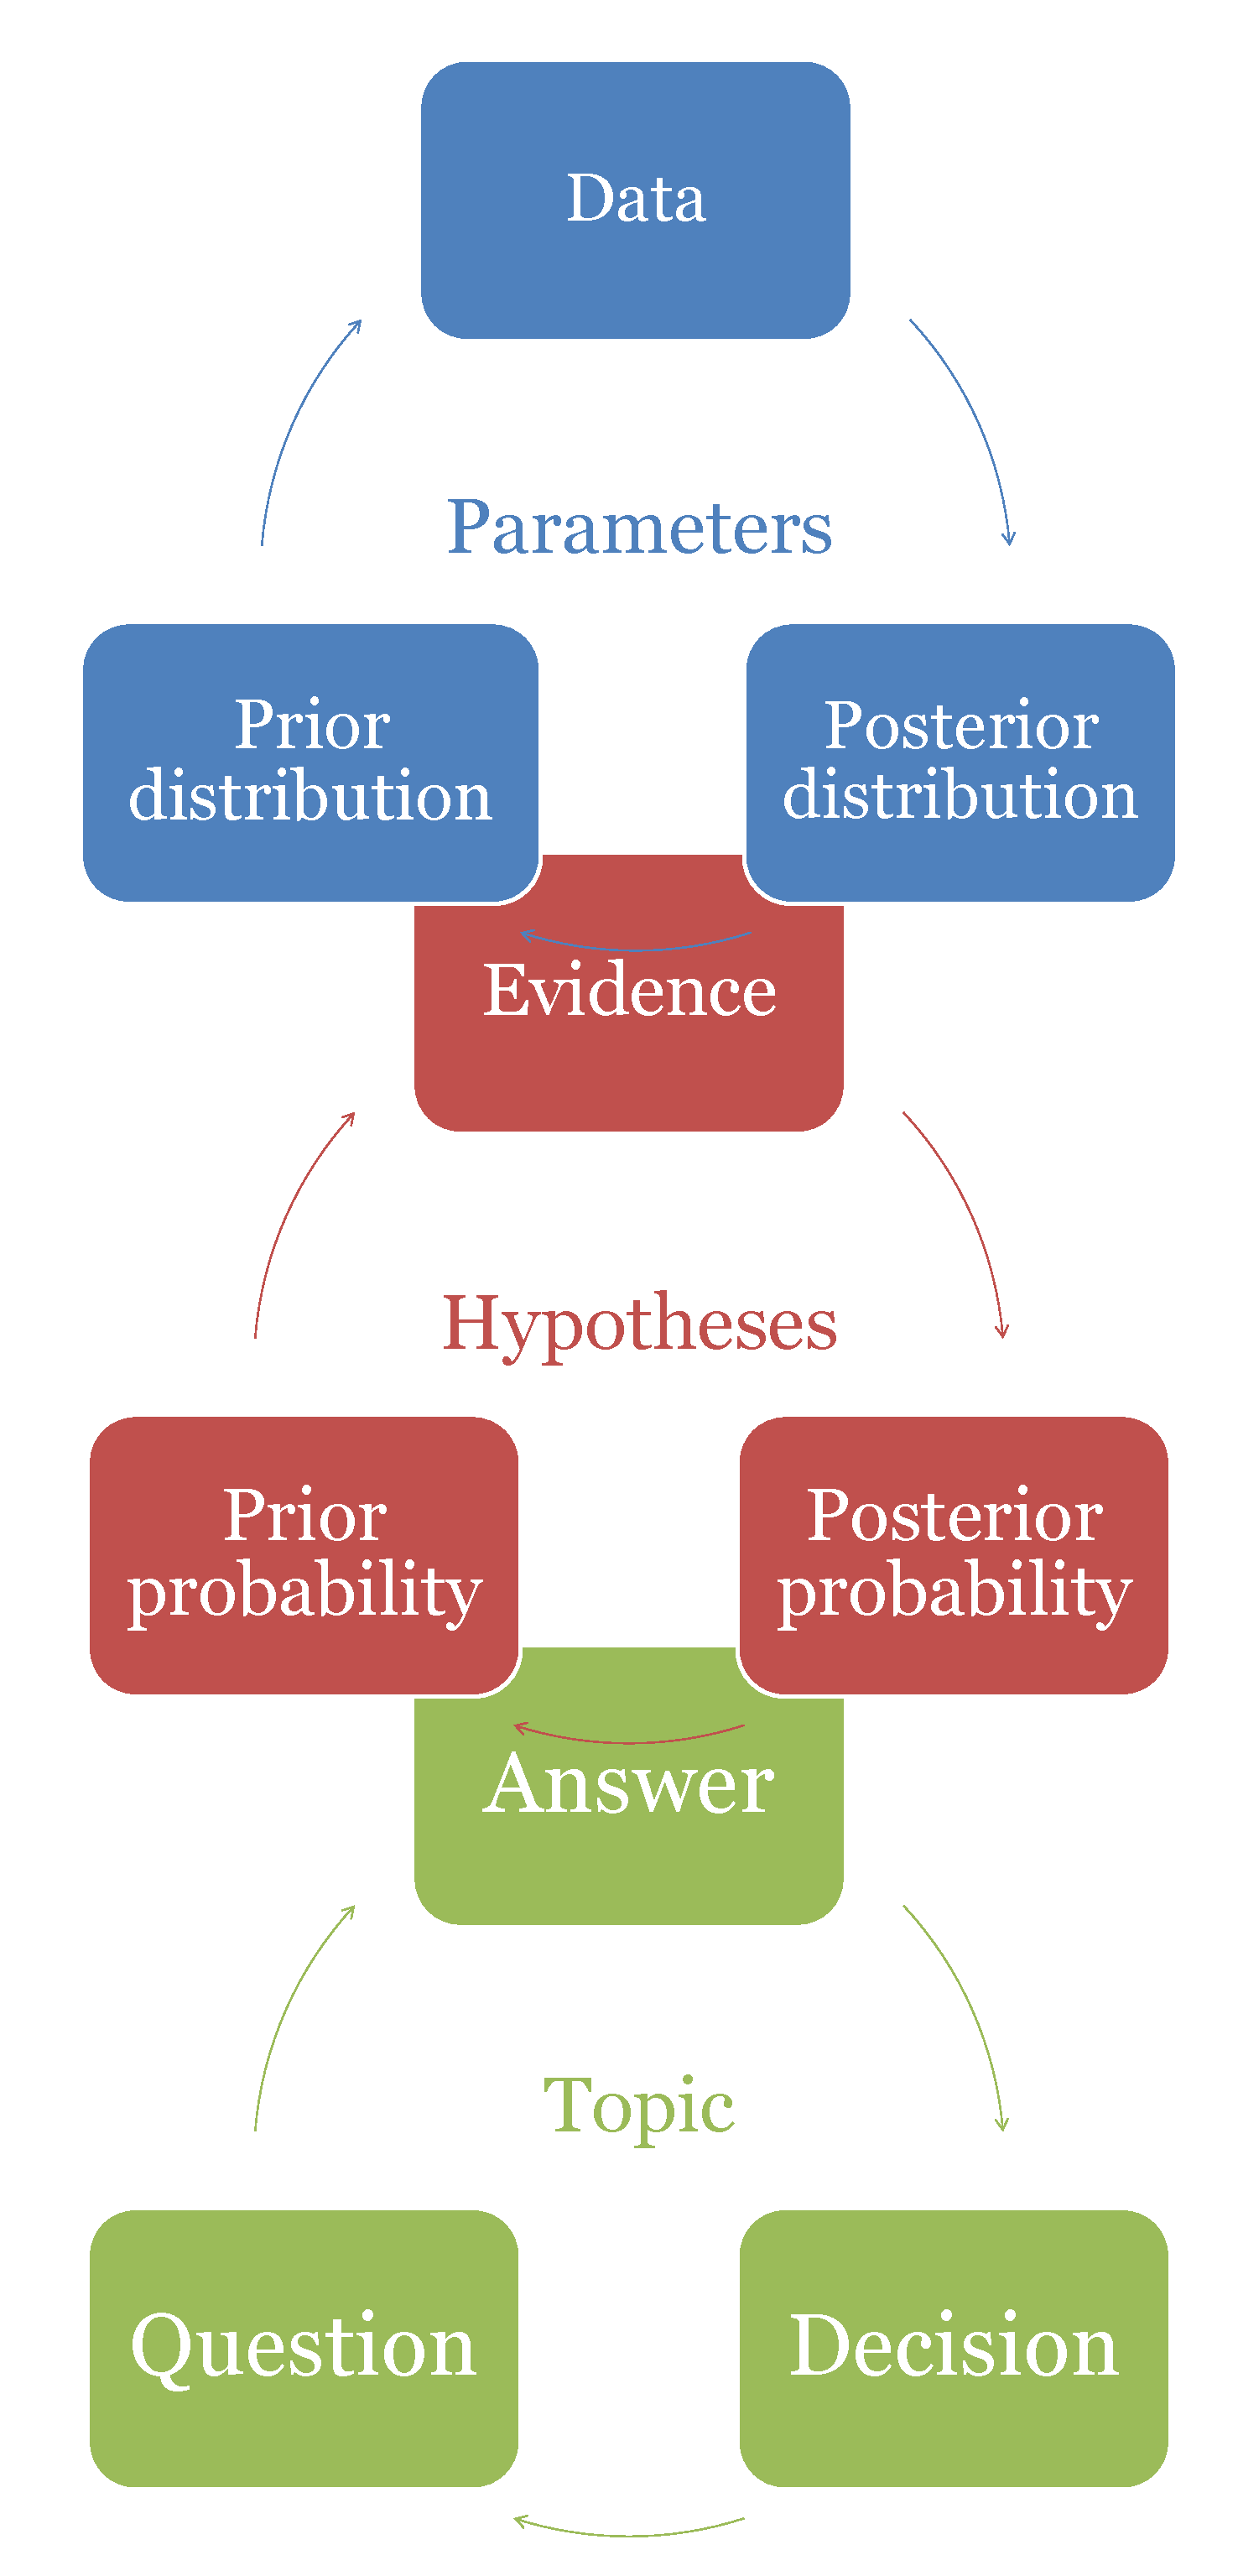
\includegraphics[width = .5\linewidth]{Figures/Figure1.pdf}
	\caption{Three updating cycles. The top cycle depicts how data is used to update a prior into a posterior distribution of parameters. The middle cycle depicts how evidence obtained using the top cycle is used to update prior probabilities into posterior probabilities of hypotheses. Finally, the bottom cycle depicts how a research question can be answered and acted upon using the posterior probabilities from the middle cycle.}
	\label{fig:loops}
\end{figure}
Parallel in the cycles is some state of prior knowledge that is updated with data, evidence or an answer, into posterior knowledge.
The actual updating step links the cycles together.

\textsc{The bottom loop} of Figure~\ref{fig:loops} illustrates updating at the level of theories.
Specifically, it shows that by answering a research question new questions are generated.
To illustrate this updating cycle, let us consider dr. Jones, a researcher who investigates the prevention of headaches.
Currently, she is interested in the question whether a new drug is an effective headache cure.
After her first research indicates that the new drug is likely effective against headaches, dr. Jones develops new research questions about the size of the effect and the side effects of the new drug.
Before being able to update her research question and theories, she needs to answer her initial research question.

\textsc{The middle loop} of Figure~\ref{fig:loops} shows that an answer can be obtained by updating knowledge about a set of hypotheses.
Dr. Jones expects that a new drug performs better than paracetamol, which in turn outperforms the placebo.
Alternatively she also considers the possibility that paracetamol outperforms both the placebo and the new drug.
She translates these expectations into two hypotheses: $H_1: \text{effect new drug} > \text{effect paracetamol} > \text{effect placebo}$ and $H_2: \text{effect paracetamol} > \{ \text{effect new drug, effect placebo} \}$.
Note that dr. Jones' expectations describe orderings ($>$ and $<$ denote larger than and smaller than, respectively) between group means rather than equalities like in a null hypothesis.
The remainder of this paper is illustrated with such inequality constrained -- informative -- hypotheses \cite{hoijtink12book,klugkist05}.
Updating knowledge at the level of hypotheses can be illustrated by means of Bayes' theorem (Equation~\ref{eq:BayesTheorem}):
\begin{align}
\label{eq:BF}
\begin{split}
%\dfrac{P(H_1)}{P(H_2)}  & \times  \dfrac{P(D|H_1)/P(D)}{P(D|H_2)/P(D)}  \\
\dfrac{P(H_a)}{P(H_b)}  & \times  \dfrac{P(D|H_a)}{P(D|H_b)}  =  \dfrac{P(H_a|D)}{P(H_b|D)},
\end{split}
\end{align}
where $P(H_a)$ is the prior probability of $H_a$, $a,b = 1,2,...,I$, $a\neq b$ and $I$ is the number of considered hypotheses, $P(D|H_a)$ is the marginal likelihood of data $D$ under $H_a$ and $P(H_a|D)$ is the posterior probability of $H_a$. 
The ratios of prior and posterior probabilities are also called the prior and posterior odds, respectively. 
The ratio of two marginal likelihoods is commonly called a Bayes factor \cite{kass95}, such that $BF_{ab}$ quantifies the relative evidence for $H_a$ and $H_b$.
Equation~\ref{eq:BF} can also be written as:
\begin{align}
\text{PrO}_{ab}  & \times  \text{BF}_{ab} =  \text{PoO}_{ab},
\end{align} 
that is, the prior odds PrO$_{ab}$ are updated with $BF_{ab}$ -- the relative belief in the two hypotheses after observing data $D$ -- into the posterior odds PoO$_{ab}$.

This evidence describes the rate with which the relative belief in two hypotheses changes.
Dr. Jones needs to quantify her knowledge about the two hypotheses into prior probabilities to obtain the posterior odds that answer her research question.
The goal of this paper is to provide a definition of what these prior probabilities are and present a procedure of how to obtain them.
For now let us assume dr. Jones knows the prior probabilities she wants to update them with the marginal likelihoods.


\textsc{The top loop} of Figure~\ref{fig:loops} shows that the evidence can be obtained by updating knowledge about a set of parameters.
Dr. Jones considers parameters $\theta_{\text{paracetamol}}$, $\theta_{\text{placebo}}$ and $ \theta_{\text{new drug}}$ in her hypotheses, where $\theta$ denotes the mean reduction in headache complaints in the respective groups, such that her hypotheses now are:
\begin{align}
\label{eq:h1}
H_1: \theta_\text{new drug} > \theta_\text{paracetamol} > \theta_\text{placebo}
\end{align}
and
\begin{align}
\label{eq:h2}
H_2: \theta_\text{paracetamol} > \{ \theta_\text{new drug} \theta_\text{placebo} \}
\end{align}
Bayes' theorem can again be used to show that a marginal likelihood $P(D|H)$ can be computed with:
\begin{align}
\label{eq:marginal}
\begin{split}
P(D|H) &= \dfrac{P(\theta|H) \times P(D|\theta,H)}{P(\theta|D, H)}
%P(D|H)& = \int P(\theta|H) \times P(D|\theta,H) d\theta\\
\end{split}
\end{align}
where $P(\theta|H)$ is the prior distribution for a set of parameters $\theta$ that quantifies the knowledge about $\theta$ before collecting any data, $P(\theta|D,H)$ is the posterior distribution of these parameters and $P(D|\theta,H)$ is the density of the data.
Equation~\ref{eq:BF} showed how a ratio of marginal likelihoods is required to update prior odds in to posterior odds. 
Equation~\ref{eq:marginal} shows that each of these marginal likelihoods depend on the prior and posterior distribution on the parameters. 
This demonstrated how updating the prior distributions of parameters into posteriors is required for the updating of the prior odds into posterior odds, which in turn are required to answer a research question.

Before she can update her knowledge dr. Jones needs to 1) formulate her initial theories and hypotheses, 2) specify prior probabilities and 3) define prior distributions for each hypothesis.
Dr. Jones can rely on APA guidelines to help her in formulating theories and hypotheses.
It is common practice to justify a research question with a literature review \cite<e.g.>[p.27-28]{apa}.
Additionally dr. Jones' hypotheses depend on, amongst others, her background, experience, colleagues.
Another researcher working in a different country, collaborating with other researchers or with more experience in the field, might develop different hypotheses.
To define the prior distributions for the parameters, dr. Jones can rely on extensive literature, ranging from methodological perspectives
\cite<e.g.>{gelman08, mulder14}
to tutorials 
\cite<e.g.>{garthwaite05, ohagan06book}
and reviews 
\cite<e.g.>{ohagan12}.

Guidelines for the specification of prior probabilities are scarce.
While articles about updating Bayes factors discuss the importance of prior probabilities, recommendations for how to specify them lack \cite{mulder14,villa15}.
Mostly no prior probabilities are considered \cite<e.g.>{hout14,maanen16} or equal prior probabilities are considered under the assumption that all hypotheses are equally likely a priori \cite<e.g.>{kopp16,rac16}.
Mostly, Bayes factors are reported and interpreted as the increase in prior odds, without reporting the corresponding prior probabilities.
These prior probabilities are required to complete the updating cycle at the hypotheses level, but also to update the complete set of nested updating cycles to answer the general research question (Figure~\ref{fig:loops}).

This paper presents a definition of prior probabilities and an elicitation procedure to specify and justify prior probabilities.
The first part of this paper discusses the middle loop of Figure~\ref{fig:loops} in more detail. The Bayes factor is further introduced, and a definition is developed of what a prior probability is.
Three meaningful components are distinguished: possibility (the probability of a hypothesis occurring, disregarding context), plausibility (the probability of a hypothesis occurring incorporating context based prior knowledge) and value (all factors that affect whether a hypothesis is considered by a researcher).
Existing approaches on the specification of prior probabilities are evaluated and compared using these three concepts.
The second part of this paper discusses an elicitation procedure executed with ten applied researchers.
The results of this procedure demonstrate that applied researchers can define sensible prior probabilities using possibility, plausibility and value and how prior probabilities differ over persons, contexts and hypotheses.

\section{What is a prior probability?}
The goal of Bayesian hypothesis testing is to find the best hypothesis from a set of hypotheses.
Consider the $j=1,...,J$ infinitely many potential hypotheses, of which only a subset $i=1,...,I$ is considered in a research project.
Let us define that a prior probability $P(H_i)>0$ quantifies that $H_i$ is considered and that $\sum_{i = 1}^{I} P(H_i) = 1$.
To develop an idea of what a prior probability represents, let us consider the reasons for considering a hypothesis.

\noindent\textbf{Reason 1.} 
\textsc{A hypothesis should be possible.}
A hypothesis is possible (i.e., it is not impossible) if it has a probability of occurring larger than $1$, disregarding the context of the hypothesis.
Possibility quantifies the proportion of the parameter space a hypothesis encompasses and can take on values between $0$ and $1$.
This definition of possibility resembles that of the complexity in the computation of Bayes factors for inequality constrained hypotheses \cite{klugkist05}.

\subsection{Intermezzo: the Bayes factor for inequality constrained hypotheses}
\citeA{klugkist05} show that the Bayes factor for inequality constrained hypotheses can be computed without evaluating the marginal likelihoods.
This approach makes use of the fact that both $H_1$ and $H_2$ are nested under the same unconstrained hypothesis $H_u: \theta_{\text{new drug}}, \theta_{\text{paracetamol}}, \theta_{\text{placebo}}$ that does not constrain the parameters in any way.
If the prior parameter distributions for the parameters in $H_u$ are considered independent and the constrained parameters get the same diffuse prior, $BF_{12}$ can be computed using the following equation \cite{klugkist05}:
\begin{align}
\label{eq:complexityfit}
\begin{split}
BF_{ab} = \dfrac{f_a/c_a}{f_b/c_b}
\end{split}
\end{align}
where $f_a$ is the fit of the data to $H_a$, that is, the proportion of the unconstrained posterior distribution in agreement with the constrained hypothesis $H_a$ and $c_a$ is the complexity of $H_a$, that is, the proportion of the unconstrained posterior distribution in agreement with the constrained hypothesis $H_a$.
If the parameters in the unconstrained prior are independent (not correlated), each of the $3!=6$ orderings of the three means is equally likely. 
Since $H_1$ is in agreement with one of these orderings, the complexity of $H_1$ is $\frac{1}{6}$.
Two orderings agree with $H_2$, rendering $c_2 = \frac{1}{3}$.
After collecting data, dr. Jones can determine the fit of her hypotheses and compute the Bayes factor, that can be used to obtain the posterior probabilities and answer her question.

Possibility resembles the concept of complexity for inequality constrained hypotheses.
An example of an impossible hypothesis is $H_{\text{impossible}}: \theta_1 > \theta_2 > \theta_3 > \theta_1$. 
This hypothesis requires $\theta_1$ to be larger and smaller than $\theta_2$ and $\theta_3$, which cannot be realized.
In contrast, the unconstrained hypothesis $H_u: \theta_1, \theta_2, \theta_3$ is always true an has a probability of $1$.
Dr. Jones' inequality constrained hypotheses cover only a part of the parameter space.

\noindent\textbf{Reason 2.} 
\textsc{A hypothesis should be plausible.}
Plausibility refers to the probability that a hypothesis occurs based on context dependent prior knowledge about the parameters.
For inequality constrained hypotheses, the concept of plausibility can also be thought of as \textit{prior fit}, that is, how well does the hypothesis fit the prior knowledge.
This prior knowledge can be informed by previous experience of the effects or conditions studied or theoretical extrapolation.
An example of an implausible hypothesis is $H_{\text{implausible}}: \theta_{\text{placebo}} > \theta_{\text{new drug}} > \theta_{\text{paracetamol}}$.
This hypothesis is possible, but current knowledge about placebos and paracetamol tells us that this hypothesis is fairly implausible.

Dr. Jones considers her knowledge about $H_1: \theta_\text{new drug} > \theta_\text{paracetamol} > \theta_\text{placebo}$ and $H_2: \theta_\text{paracetamol} > \{ \theta_\text{new drug}, \theta_\text{placebo} \}$.
She concludes that little is known about the effectiveness of the new drug, but previous research shows that paracetamol certainly outperforms placebos.
Based on this knowledge she assigns $H_1$ a plausibility of $1/3$.
The process of how knowledge is translated into a plausibility will be the topic of discussion in section Prior probability elicitation.
While assigning a plausibility to $H_2$, dr. Jones is unsure of the relative effectiveness of paracetamol and new drug, which combined with the knowledge of paracetamol and placebo results in a plausibility of $.75$.

\noindent\textbf{Reason 3.} 
\textsc{A hypothesis should be valued.}
Both possibility and plausibility contribute to how much a hypothesis is valued by a researcher.
Possibility and plausibility can vary between hypotheses.
A possible hypothesis can be very implausible and vice versa.
For example, it is possible that the placebo will outperform both the new drug and paracetamol in preventing headaches, but it is not plausible.
Alternatively, consider comparing paracetamol to not only the new drug and a placebo, but also to eating an apple, candy, a kiss on the forehead, an ice-bath and drinking a beer.
While it is very plausible that paracetamol outperforms all of the alternative `treatments', this expectation describes only $1.56\%$ of the total parameter space.
While this hypothesis has high plausibility, it has low possibility.
The combination of possibility and plausibility in part explains why hypotheses are considered.
If a hypothesis is neither possible nor plausible, it is unlikely to be considered.
If a hypothesis is both possible and plausible, it might not be considered because it is considered redundant.
After all, if a hypothesis has a high possibility, it is not very specific and not much can be learned from this hypothesis. 
If additionally, the plausibility of this hypothesis already is high, it might not be worth time and resources to learn more about this hypothesis.

Possibility and plausibility alone cannot fully explain why some hypotheses are considered, while others are excluded. 
Consider a researcher who wants to prove or disprove an established theory, for example: the world is flat versus the world is round. 
While there are many alternative hypotheses that are more possible and plausible than 'the world is flat', they do not reflect the researcher's aim and thus are not considered.
The considerations for investing time and resources and thus to include a hypothesis cannot be attributed only to the possibility and plausibility of a hypothesis.
Dr. Jones considers $H_1$ and $H_2$ because they are possible and plausible, and because she is particularly interested in the effectiveness of the new drug relative to paracetamol.
For example, $H_{\text{not valued}}: \{ \theta_{\text{paracetamol}},\theta_{\text{new drug}} \} > \theta_{\text{placebo}}$ is both possible and plausible but dr. Jones does not consider this hypothesis because it makes no prediction on the relative effectiveness of paracetamol and the new drug.

\section{Prior probability specification}
A prior probability quantifies how much a hypothesis is valued while taking into account its possibility and plausibility.
Guidelines and recommendations for specifying prior probabilities are sparse in the literature, and at best vague \cite{villa15}.
The paragraphs below discuss how different approaches to prior probability specification include possibility, plausibility or value in their definition and how feasible the approach is.

\subsubsection{No prior probabilities}
A common practice in Bayesian hypothesis testing is to not specify any prior probabilities and focus on the Bayes factor \cite<e.g.>{wetzels12, hout14}.
The Bayes factor can be interpreted as the strength of evidence, or as the rate with which the prior beliefs need to be adjusted \cite{mulder16}.
Guidelines have been proposed to classify the strength of evidence in verbal categories \cite<e.g.>{kass95,wagenmakers11} that take focus away from the prior odds.
\textit{After Dr. Jones completes her research, she computes a Bayes factor and finds that $H_1$ is $4$ times more supported by the data than $H_2$.
She concludes that $H_1$ is preferred with substantial evidence \cite{wagenmakers11}.
She does not report any prior or posterior probabilities.
}

If no prior probabilities are considered, the conclusion is only affected by the data and not by prior knowledge.
This approach does not incorporate possibility, plausibility or value, because prior probabilities are not considered.
Limiting the conclusion to the level of evidence (Bayes factor), without updating prior probabilities is equivalent to using equal prior probabilities.

\subsubsection{Equal prior probabilities}
An easy way to obtain posterior probabilities is to assign equal prior probabilities to all hypotheses \cite<e.g.>{jarosz17}.
A simple calculation transforms any set of Bayes factors into posterior probabilities.
\textit{Dr. Jones transforms the Bayes factor using equal prior probabilities ($P(H_1)= P(H_2) = .5$.
If the Bayes factor is $4$, the posterior probabilities of $H_1$ and $H_2$ are $.8$ and $.2$ respectively.
This tells her nothing more than what she knew already: that $H_1$ is $4$ times more supported by the data than $H_2$.
}

Using equal prior probabilities is equivalent to interpreting only the Bayes factors \cite{kruschke18}.
Neither of these methods uses any prior information.
\citeA{mulder14} advises to use equal prior probabilities only when absolutely no prior knowledge is available.
When a researcher considers equal prior probabilities without further explanation it is unclear whether this reflects the prior knowledge or is just a default choice.
Furthermore, it is very unlikely that all considered hypotheses are exactly equally probable a priori.
Using equal prior probabilities is often used as a quick and default way to obtain posterior probabilities.

\subsubsection{Complexity as prior probability}
In Section 1.6 \citeA{Jeffreys1961} elaborates the idea that simpler hypotheses should always have a larger prior probability than hypotheses that are more complex.
The concept complexity was introduced in the context of inequality constrained hypotheses in the section What is a prior probability? 
It is a measure of how constrained a hypothesis is, relative to the unconstrained hypothesis.
Using complexity as a prior probability implies that equally constrained hypotheses receive the same prior probability \cite{scott10}.
\textit{Dr. Jones considers complexity as the prior probability.
		She determines that $P(H_1) = 1/6$ and $P(H_2) = 1/3$ based on the proportion of the parameter space they cover.}
Equation~\ref{eq:complexityfit} showed that a Bayes factor for inequality constrained hypotheses can be written as a ratio of the fit of a hypothesis divided by its complexity.
If the relative prior complexities are used as the prior odds and multiplied with the Bayes factor, which also contains the complexities, these cancel out and the resulting posterior odds are the relative posterior fits of the data to the model:
\begin{align}
\label{eq:nocomplexity}
\begin{split}
\dfrac{c_a}{c_b} \times \dfrac{f_a/c_a}{f_b/c_b} = \dfrac{f_a}{f_b}
\end{split}
\end{align}

\subsubsection{Prevalence as prior probability}
\citeA{ioannidis05,wilson18} suggest to use the relative prevalence rate of true hypotheses in a particular field as prior odds.
Although counting the number of rejected hypotheses in a field seems like a straightforward procedure to gain knowledge about the objective plausibility of a hypothesis, three potential problems might arise.
The first problem is defining the field to derive the odds from. 
Dr. Jones could consider all research on paracetamol, or all research on headache prevention, or all research on new versus established medication, or many other definitions of the `field'.
The second problem is that the available literature might not be a good representation of all conducted research.
Publication bias creates an over-representation of significant findings in the literature \cite<e.g.>{Rosenthal1979,ioannidis05}.
It is difficult to know by what factor the observed prevalence is overestimated.
Finally, it is unclear how to observe the prevalence of informative hypotheses that might include combinations of (in)equality constraints and have not been considered previously.
\textit{Dr. Jones investigates the literature and finds that over $1,000$ articles consider hypotheses similar to $H_2$ but only in about $5\% = 50$ of these papers is this hypothesis compared to a hypothesis like $H_1$. 
Only two of these studies have $H_1$ as the preferred hypothesis, and $17$ prefer $H_2$. 
The remaining $31$ papers prefer another considered hypothesis or are indecisive.
Dr. Jones does not know how to translate this information into prior probabilities for her hypotheses.
}


\subsubsection{Subjective prior probabilities}
\citeA{morey16phil, rouder16} argue in favor of defining subjective prior probabilities, that is, prior probabilities that reflect the prior beliefs of a researcher.
\citeA{tijmstra18} also pleas for using plausibility as a reasonable prior probability.
Choosing a prior probability based on the subjective beliefs of a researcher aligns with the definition of a prior probability provided in this paper.
However, no methods are available for applied researchers to translate their knowledge in to a meaningful prior probability.
\textit{Dr. Jones thinks about her prior beliefs of $H_1$ and $H_2$, and finds it difficult to quantify her beliefs about these hypotheses.}

\subsubsection{Betting odds as prior odds}
\citeA{hofstee84} has proposed a betting framework to think about the probabilities of hypotheses.
Researchers should justify the hypotheses they choose to consider by placing a bet on the possible outcomes.
\textit{Dr. Jones considers her hypotheses and decides to bet with a rate of $6:2$ on the hypotheses.
From this quantification we determine that her prior probability of $H_1$ is three times larger than that of $H_2$.
When she wants to report these prior odds, she has trouble explaining what made her choose these specific odds.}
If hypotheses are valued differently, the betting odds chosen for these hypotheses will differ.
However, it is not formally described how these betting odds could be derived or defended.
Similar to the consideration of subjective prior probabilities, it is unclear how a bet should be placed and how a researcher could justify the bets.

\subsection{What is a prior probability?}
The presented approaches for specifying a prior probability all seem to incorporate one or more of the reasons to consider a hypothesis (possibility, plausibility, value).
If an approach used plausibility or value it is unclear how to actually quantify this.
The possibility, plausibility and value together describe the prior belief in a hypothesis.
The next section presents an elicitation procedure developed to elicit the possibility and plausibility for hypotheses and use this quantified knowledge to express how they value their hypotheses by betting on them.

\section{Prior probability elicitation}
A procedure was developed to elicit the prior probabilities of hypotheses.
Thirteen behavioral researchers were approached to participate in an experiment in which the procedure was executed.
The researchers were non-randomly selected, utilizing the network of the author within Utrecht University.
A requirement for selection was familiarity with Bayesian hypothesis testing and informative (inequality constrained) hypotheses.
Familiarity with Bayesian factors limits necessary explanations on Bayesian statistics, updating or prior odds.
Familiarity with informative hypotheses ensures that researchers have encountered hypotheses of varying complexity before.
Of the thirteen approached researchers, ten were available within the set time frame of two months (April and May 2018).

The elicitation procedure consisted of explanation and questions divided in two main parts: a Training Phase, where participants learn new concepts and procedures and a Test Phase, where the learned procedure is applied to new contexts.
The whole procedure lasted approximately one hour for each participant.
Participants could at any point ask for clarification or guidance, and were informed that not their knowledge, but the procedure was under evaluation. 
Any questions or comments were answered during the elicitation by the author.

The elicitation procedure serves three goals.
The first goal is to evaluate whether possibility, plausibility and value can be elicited and distinguished.
This is achieved by introducing a stepwise elicitation procedure.
This stepwise method is introduced to the participants after familiarizing participants with assigning probabilities to hypotheses and refreshing or extending their knowledge on Bayesian updating.
The second goal of the experiment is to demonstrate that researchers are able to use the learned procedure and concepts to elicit prior probabilities for hypotheses that do not concern their own research and to their own hypotheses.
The third and final goal of the experiment is to evaluate whether the procedure is a valid method to elicit prior probabilities. 
Throughout the elicitation procedure evaluation questions are asked.
The results of these goals are presented in the next three sections.

\section{Eliciting and distinguishing possibility, plausibility and value}
The previous section introduced three concepts that each describe part of a prior probability: possibility, plausibility and value.
The first goal of the elicitation procedure is to demonstrate that each of these concepts can be elicited.
The sections below present those parts of the procedure that demonstrate the elicitation possibility, plausibility and value.
The full procedure is available on https://github.com/fayetteklaassen/prior-probabilities.


\subsection{Possibility}
The possibility of a hypothesis, as discussed before, relates to the proportion of the parameter space covered by the hypothesis.
To elicit this, participants are introduced to four hypotheses about parameters $a$, $b$ and $c$.
They are informed these letter represent three group means, without any further context.
The hypotheses describe expected orderings between two or three of these means (see the first column of Table~\ref{tab:hypsExperiment}).
\begin{table}
\begin{tabular}{ l l l l}
	\hline
	 &No context & Headache & Flanker \\
	\hline
	$H_1$& $a > b$ ; $c$ & paracetamol > placebo & uniform > contrast\\
	$H_2$ &$  a > c$ ; $b$&paracetamol > apple &  control > uniform\\
	$H_3$ &$  a > b > c$&  paracetamol > placebo > apple & uniform > control > contrast\\
	$H_4$ &$ c > b> a$&  apple > placebo > paracetamol & control > uniform > contrast\\
	\hline
\end{tabular}
	\caption{Hypotheses considered at three steps in the elicitation procedure. The column \textit{No context} shows the hypotheses presented to participants before context was available. The column \textit{Headache} shows the hypotheses in the Headache example, and the Flanker column shows the hypotheses in the }
	\label{tab:hypsExperiment}
\end{table}

Researchers are instructed to consider each hypothesis separately and specify a probability between $0$ and $1$ that describes how likely it is that the hypothesis is true versus that it is not true.
The possibility of a hypothesis could be derived without elicitation, but this step is explicitly introduced to facilitate the elicitation of plausibility in the next step.
Participants are taught to think of possibility in terms of the number of possible orderings between parameters.
Both $H_1$ and $H_2$ constrain only two parameters, while $H_3$ and $H_4$ constrain all three parameters.
The assigned probabilities to the hypotheses are displayed in the first column in Figure~\ref{fig:probapple} labeled possibility\footnote{Note that the presented probabilities are rescaled so that their sum adds up to 1.}.
The hypotheses were chosen such that $H_1$ and $H_2$ should be equally possible and more possible than $H_3$ and $H_4$.
The results show that these $10$ researchers managed to quantify the possibility of four inequality constrained hypotheses without any context about these hypotheses.

\subsection{Plausibility}
Plausibility of a hypothesis relates to the knowledge about the parameters.
To elicit this, context is added to the example, such that participants can activate their knowledge.
The same four hypotheses are considered, but now in the fictional context of a researcher who is interested in preventing headaches (right column of Table~\ref{tab:hypsExperiment}).
This randomly assigns patients to one of three treatments: a paracetamol ($a$), a placebo ($b$) or an apple ($c$) and measures their headache level the next day.
The researchers are asked to consider the hypotheses once more and assign to each hypothesis a probability that it is true versus that it is not true, incorporating their knowledge about the headache prevention ability of paracetamol, placebo and apples.
These probabilities are presented in the second column of Figure~\ref{fig:probapple} labeled plausibility.
The plausibility assigned to the hypotheses differs from the possibility of the hypotheses.
Specifically, $H_3$ generally is considered more plausible than possible.
This is reasonable because $H_3$ almost perfectly describes the common perceptions of the effectiveness of paracetamol, placebos and apples.
Additionally, $H_3$ is never assigned a higher plausibility than $H_1$.
This is a consequence of the fact that $H_3$ is nested in $H_1$, that is, $H_1$ has a higher possibility.
Figure~\ref{fig:probapple} shows that the plausibility assigned by researchers aligns with what can be expected based on common knowledge.
It shows that for a research example where knowledge is considered fairly similar between people, the elicited plausibility indeed is rather stable over participants.
Additionally, there is a clear differentiation between the assigned possibility and plausibility, where some hypotheses are assigned higher plausibility than possibility after learning the context, and for other hypotheses the reverse is observed. 

\subsection{Value}
For the elicitation of possibility and plausibility researchers were asked to consider each hypothesis in itself.
To evaluate whether value plays a role besides possibility and plausibility, the hypotheses are considered as a set.
Three tasks in the experiment ask researchers to bet on the hypotheses, to literally measure how they value the hypotheses.
In the first task, participants are instructed to consider only the possibility they assigned to the four hypotheses before any context is added (that is, the hypotheses in the first column of Table~\ref{tab:hypsExperiment}), and consider the possibility in placing their bets.
The results are presented in Figure~\ref{fig:probapple}. 
The placed bets are in line with what can be expected. 
Because $H_1$ and $H_2$ have the highest possibility, the expected pay-out for these hypotheses is highest, and there is no differentiation between the two hypotheses.
Some participants choose to bet on the hypotheses with lower possibility too, but with lower bets.
Finally, participant $6$ bet on $H_3$ but not on $H_4$.
This researcher might value $H_3$ and $H_4$ differently for how they relate to the other two hypotheses considered.
This first task demonstrates that researchers already differ in how they translate the value of possibility into a bet.
Even though the expected value for $H_1$ and $H_2$ is highest, some people choose to bet on $H_3$ and $H_4$ also.
These hypotheses might be valued because they provide the potential knowledge gained by investigating these hypotheses.

In the second task, participants again consider the hypotheses without any context, and consider the knowledge gain of each hypothesis in addition to the possibility.
The knowledge gain is determined by taking the inverse of the possibility, and is presented in the form of a betting odds.
That is, a hypothesis with a possibility of $.5$ is assigned a betting odds of $1/.5 = 2$.
The betting odds tell how many times a bet is paid out if that hypothesis is in fact the best hypothesis and are a quantification of how much knowledge is gained by learning about this hypothesis.
The placed bets are considered 
Participants are asked to consider these betting odds and the possibility they assigned to the hypotheses in placing their bets.
If only the possibility of a hypothesis (transformed into the betting odds) affects how researchers bet on a set of hypotheses, the relative bets for the four hypotheses would be all equal.
Consider $.5$ and $.25$ as the possibilities of two hypotheses. 
Their respective betting odds would be $2$ and $4$.
The expected pay-out for each hypothesis is $.5\times2=1$ and $.25\times4=1$, which corresponds to an expected equal bet on the two hypotheses.
The fourth column of Figure~\ref{fig:probapple} shows the bets placed on the four hypotheses.
While participants $1$, $4$, $5$ and $7$ indeed distribute their bets equally, the bets of participants $2$, $6$ and $10$ resemble their assigned possibilities.
In other words, these participants only considered the possibility in placing their bets.
Participants $3$ and $8$ seemed to consider only the betting odds in placing their bets, betting more on the hypotheses that pay out more (provide more knowledge).
Finally, participant $9$ considered even a different approach, betting most on $H_2$ and $H_4$.
While there is no numerical reason to make this particular bet, it appears this participant considers something more than the possibility and the knowledge gain of the hypotheses.
The reason might be that the comparison of $H_2$ and $H_4$ seems the most interesting to this researcher.
This second task demonstrates that researchers show different betting behavior that cannot uniquely be attributed to possibility or the gain in knowledge.

Plausibility too can play a role determining the prior probabilities of hypotheses.
The third task asks researchers again to place a bet on the hypotheses, taking the betting odds and plausibility of the hypotheses into account and how they value the hypotheses.
Similar to the previous task, the expected pay-off can be computed, by multiplying the betting odds (the pay-out) with the plausibility (the subjective probability that the hypothesis is true).
The expected value is presented in the fifth column of Figure~\ref{fig:probapple}, and the sixth column presents the actual placed bets.
For participants $2$, $5$, $6$, $7$ and $8$, the relative ordering of placed bets resembles the prediction.
Only the size of the bets deviates from the prediction.
The bet placed on $H_4$ is higher than expected for participants $4$ and $9$, indicating that this hypothesis is valued more than expressed by only the possibility and plausibility.
Even though the participants have similar knowledge on the effectiveness of paracetamol, placebo and an apple in preventing headaches, the final bets are widely different from each other and from the expectation if only possibility and plausibility are taken into account.
It appears that the hypotheses are valued differently by different researchers.

The Training Phase shows three things.
First, it shows that ten researchers were able to specify the possibility of four hypotheses.
Second, after adding a context to the hypotheses researchers specify the plausibility of hypotheses.
The added context affects the variability of the individual answers, indicating that the plausibility of hypotheses differs from person to person, albeit slightly.
Finally, when asked to placed bets incorporating only possibility or both possibility and plausibility, the placed bets differ from expected bets, indicating that individuals value the hypotheses differently.
The final bet placed is an elicited prior probability.
In this prior probability, researchers are given the opportunity to include the possibility, plausibility and their value of the hypotheses.


\begin{figure}
	\includegraphics{Figures/probApple.pdf}
	\caption{Assignment of possibility, plausibility and bets to the hypotheses without and with context for the headache example (see Table~\ref{tab:hypsExperiment}). Each row depicts a participant. The columns show (1) Possibility; (2) Plausibility; (3) Bet 1, incorporating possibility; (4) Bet 2, incorporating possibility and betting odds; (5) Prediction, the predicted bet based on betting odds and plausibility; (6) Bet 3, incorporating betting odds and plausibility.}
	\label{fig:probapple}
\end{figure}

\section{Eliciting probabilities}
The second goal of the elicitation procedure is to evaluate whether researchers can use the procedure to assign probabilities in practice.
This is achieved by two final tasks in the experiment.
In the first task participants are asked to consider four hypotheses about a psychological phenomenon, that is not their own research interest.
This task mimics the scenario where researchers are confronted with hypotheses and evidence of another researcher and have to define their own probabilities to evaluate this evidence.
The second task asks researchers to formulate two or more hypotheses about their own research.
They complete the procedure for this set of hypotheses, resulting in their own prior probabilities.

The hypotheses presented by a hypothetical other researcher concern an adaptation of the Flanker task \cite{Eriksen1974}.
In this fictional reaction time experiment, participants are asked to identify the middle letter in a sequence of five letters as an X (press left hand key) or an O (press right hand key) as quickly as possible.
Three conditions are considered: Uniform -- the target letter is flanked by copies of the same letter (e.g. XXXXX), Contrast -- the target letter is flanked by copies of the contrasting target letter (e.g. XXOXX) and Control -- the target letter is flanked by copies of a lower case letter that is different from the target letters (e.g. ssOss).
Four hypotheses are formulated about the average reaction time in the correct trials for each of these conditions.
The four hypotheses are presented in Table~\ref{tab:hypsFlanker}.

Participants are asked to think about the probability of these hypotheses, disregarding context (possibility), the probability of these hypotheses incorporating their knowledge (plausibility) and to finally place a bet on these hypotheses.
Figure~\ref{fig:flanker} shows the results of this procedure.
The first column shows the possibility, which was given and is thus uniform over the hypotheses.
The second column presents the plausibility of the hypotheses for each participants.
The third column shows the predicted bet based on the possibility and plausibility.
Finally, the fourth column shows the actually placed bets.
For some participants the expected value does well in predicting the placed bets.
For others, the prediction does not account for the fact that some hypotheses are not considered, by betting nothing on them.
Neither the expected value nor the possibility or plausibility can explain the betting of the participants, indicating that the final probability also reflects how researchers value the hypotheses differently.

\begin{figure}
	\includegraphics{Figures/Flanker.pdf}
	\caption{Plausibility and bets assigned to the hypotheses for the Flanker example (see Table~\ref{tab:hypsExperiment}). The columns show from left to right (1) Possibility; (2) Plausibility; (3) Predicted bet based on possibility and plausibility; and (4) actually placed bet.}
	\label{fig:flanker}
\end{figure}

Finally, participants are asked to consider a set of hypotheses about their own research.
They quantify the possibility and plausibility of their bets and place their bets accordingly.
Figure~\ref{fig:ownhyp} shows, from left to right, the possibility, plausibility, predicted and placed bets.
Note that each researcher could define their own hypotheses, so the number and possibility of the hypotheses differ between participants.
In the Flanker example a bet could be withheld to express a hypothesis not valued.
In the current task, researchers already excluded all hypotheses they did not value to create their set of interest, and logically all hypotheses considered receive a bet.
Similar to the Flanker task, the relative size of the placed bets differs from the prediction, plausibility and possibility.
Even for a self-chosen set of hypotheses in a researcher's own field, plausibility and possibility cannot account for the differences in the placed bets.
Additionally, between researchers different types of bets can be observed. 
While for participant $1$, $5$ and $7$ the final bets are equal or almost equal for all hypotheses, participants $2$, $4$, $8$ and $10$ show a substantial bet on one hypothesis, while dividing a smaller amount over the remaining hypotheses.
These differences demonstrate that it seems unrealistic to develop a default rule for prior probabilities, or a rule of thumb. 
Clearly, as the context of a research question differs, the set of hypotheses changes, and so do the relative probabilities.

\begin{figure}
	\includegraphics{Figures/Own.pdf}
	\caption{Plausibility and bets assigned to a set of hypotheses defined by each participant. The number of hypotheses varies over participants. The columns show from left to right (1) Possibility; (2) Plausibility; (3) Predicted bet based on possibility and plausibility; and (4) actually placed bet.}
	\label{fig:ownhyp}
\end{figure}


\section{Evaluation of the elicitation}
The results of the elicitation presented above demonstrate that possibility and plausibility alone do not account for the prior probabilities of hypotheses.
The value of a hypothesis is also included in the placed bets.
To evaluate the elicitation method, several feedback questions were asked during the elicitation procedure.
The procedure is evaluated in terms of face validity, reliability and feasibility \cite{johnson10a}.
All measures are evaluated by means of self-evaluation on a $5$-point scale where $1$ indicates \textit{not at all} and $5$ indicates \textit{certainly}.
The main results of these questions are presented below.

Face validity is evaluated for each set of hypotheses (headache; Flanker; own hypotheses) after placing the final bets.
Participants were asked to rate on a 5-point Likert scale how well the bets they placed reflect their knowledge for the probabilities of the hypotheses, where $1$ indicates Not at all, and $5$ indicates completely.
By asking this question, researchers are invited to reflect on the input they provided so far.
It appears that researchers feel mostly that the bets they specified are a good reflection of their ideas, for the probabilities of their own hypotheses (min = $4$, max = $5$, mean = $4.65$).
The average feeling of how good ideas were reflected in the bets was also good for the headache example (min = $2$, max = $5$, mean = $4.00$) and Flanker task (min = $2$, max = $5$, mean = $4.15$).
This shows that the procedure is capable of eliciting values that reflect a researcher's ideas.
It appears more valid for the elicitation of probabilities for own hypotheses than for a mock example or research outside one's field.
In other words, the procedure has the highest face validity when determining the prior probabilities for one's own research.

Reliability too is measured after every placed bet, by asking participants to rate the following statement on the same five point Likert scale: \textit{If I were to complete this procedure again, I would obtain similar probabilities}.
For hypotheses they specified themselves, researchers were on average quite certain about their bets (mean = $4.6$, min = $4$, max = $5$).
For hypotheses about the Flanker task, participants were less certain about their own reliability (mean = $4.25$, min = $4$, max = $5$).
The self-reported reliability is high for both the prior probability of own hypotheses and for the Flanker example.
Even though it is self-reported, these results indicate the method is considered to provide reliable prior probabilities.

Finally, feasibility was measured at three moments in the experiment.
First, at the end of the Training Phase, participants are asked whether the steps were easy to execute (mean = $4.2$, min = $2$, max =$5$) and whether they feel capable to apply the used procedure (mean = $4$, min = $3$, max = $5$).
These results show that the method was easy to follow and execute, with the provided guidance.
After assigning probabilities to the Flanker hypotheses, participants are asked to reflect how capable they feel in assigning probabilities to hypotheses outside of their own field (mean = $3.3$, min = $2$, max = $5$).
Finally, after assigning probabilities to their own hypotheses participants are asked to reflect how capable they feel to assign probabilities to their own hypotheses (mean = $4.05$, min =$4$, max = $5$).
Similar to the face validity, participants feel more capable to assign probabilities to their own hypotheses than to the Flanker hypotheses.
The method might be most suitable for defining probabilities to hypotheses that a researcher has knowledge about.

\section{Discussion and conclusion}
This article has three goals.
First, by discussing the role of prior probabilities within the updating cycle, the importance and necessity of specifying prior probabilities is illustrated.
Posterior probabilities can only be obtained when prior probabilities are specified and updated with evidence.
Dr. Jones has completed the prior probability elicitation procedure, resulting in prior probabilities of $.3$ and $.7$ for  $H_1: \theta_\text{new drug} > \theta_\text{paracetamol} > \theta_\text{placebo}$ and $H_2: \theta_\text{paracetamol} > \{ \theta_\text{new drug}, \theta_\text{placebo} \}$, respectively. 
She conducts an experiment resulting in a Bayes factor $BF_{12} = 4$ and update her prior odds of $.3/.7=0.43$ into posterior odds of $1.71$.
The a priori belief of dr. Jones for $H_2$ was almost twice as large as for $H_1$.
The data do not align with this prior belief, and express a preference for $H_1$, resulting in a posterior probability of $.63$ for $H_1$ and $.37$ for $H_2$.
Dr. Jones uses the posterior probabilities to answer her research question and has completed one loop of the research cycle.

However, she is not satisfied with the current state of knowledge on the effectiveness of the new drug.
Based on the results of the first research project she has become interested in a third hypothesis $H_{3}: \{ \theta_{\text{paracetamol}},\theta_{\text{new drug}} \} > \theta_{\text{placebo}}$.
Figure~\ref{fig:loops} shows how the answer to a research question influences the decision to do further research, and develop a new research question.
This initiates a new cycle through the updating loops.
In this second cycle, the posterior odds for $H_1$ relative to $H_2$ can be used as prior odds.
Because $H_3$ is now considered in addition to $H_1$ and $H_2$, the prior odds relative to the newly considered hypothesis have to be formulated.
Also for updating the parameter cycle dr. Jones can use the posterior distribution from her first project as her new prior distribution for $H_1$ and $H_2$. 
For $H_3$, a new prior distribution has to be defined, that can be used to compute the marginal likelihood and corresponding Bayes factors.
If dr. Jones had decided to not define any prior probabilities in her first research project, she would not have been able to update this knowledge in a second research cycle, because she would fail to account for the knowledge already available from the earlier research.

The second goal of this article is to define what a prior probability is.
Assigning a prior probability to a hypothesis means to consider it, and thus to exclude the hypotheses that do not get a prior probability assigned.
Prior probabilities can be used to describe the relative prior belief for a set of hypotheses.
Three reasons determine whether a hypothesis is considered: its possibility, plausibility and value to the researcher.
Existing guidelines for the specification of prior probabilities all relate to one or more of these aspects.
The varying proposed strategies can be differentiated and summarized with these three components by means of the elicitation procedure in this paper.
Possibility, plausibility and value can each be distinguished from the results.
This seems to justify the definition of prior probabilities in terms of possibility, plausibility and value.

The third and final goal of this article is to provide a concrete guideline that allows researchers to define their own prior probabilities.
This is useful in updating knowledge in their own research, where they can then update their prior probabilities and can report the findings.
It can also be beneficial to interpret Bayes factors reported in other research based on own specified prior probabilities for the hypotheses considered.
This article presents an elicitation procedure that is directed at specifying prior probabilities following the distinction in possibility, plausibility and value.
The results show that it is possible to differentiate these three concepts between individuals, and that by manipulating context, knowledge or value, the corresponding component is affected.
Furthermore, individuals differ in their assigned prior probabilities, and rarely do equal prior probabilities represent the researchers' prior knowledge adequately.

The results also show that participants rated the procedure feasible, valid and reliable.
Both the validity and self-reported reliability were on average higher in the context of own hypotheses rather than predefined hypotheses.
This further supports the argument that it is important to report prior probabilities rather than leave it to the reader to define their own prior probabilities.
A reader can still disagree with these probabilities, but can better consider how to disagree.

This article has demonstrated how possibility and plausibility play a role in eliciting prior probabilities, but cannot explain these entirely.
How a researcher values a hypothesis relative to other considered hypotheses appears to play a role in the final prior probability assigned to it.
Through evaluation of the elicitation procedure, it appears that researchers are able to think about their own prior probabilities and report their rationale behind them, whether they use the introduced procedure or another method.
Specifying prior probabilities allows researchers to evaluate the evidence in light of their prior beliefs and reflect on the agreements, disagreements and surprises between prior beliefs and evidence from data.
This creates a more open research cycle, and enables us to be in the loop continuously.

 \clearpage
 \newpage
 \bibliographystyle{apacite}
 \bibliography{C:/Users/4104803/Surfdrive/references}	
\end{document}
